% Phase 1 -- Literature Review and Concept (4 November 2026).
% Based on the course-supplied project-proposal.tex (ACL 2015 format).
\documentclass[11pt]{article}
\usepackage{acl2015}
\usepackage{times}
\usepackage{url}
\usepackage{latexsym}
\usepackage{booktabs}
\usepackage{tabularx}
\usepackage{array}
\usepackage{float}
\usepackage{tikz}
\usetikzlibrary{arrows.meta,positioning}
\usepackage[T1]{fontenc}
\usepackage[utf8]{inputenc}

\title{Clickbait Without the Click:\\Linguistic Cues under Temporal Shift\\Project Proposal for NLP, Winter 2026/27}
\author{Igor Ko{\l}odziej, Hubert Kowalski, Adam Kaniasty, Mateusz Iwaniuk \\
Warsaw University of Technology\\
Supervisor: Anna Wr{\'o}blewska}
\date{}
\newcommand{\mF}{macro-\(F_1\)}

\newcommand{\IgorPhaseOne}{Proposal drafting (approach, evaluation, work deliverables); 4 hours}
\newcommand{\HubertPhaseOne}{Proposal drafting (approach, evaluation, work deliverables); 4 hours}
\newcommand{\AdamPhaseOne}{Literature review, source metadata audit and data scoping; 4 hours}
\newcommand{\MateuszPhaseOne}{Literature review, source metadata audit and data scoping; 4 hours}

\begin{document}
\maketitle
\begin{abstract}
We investigate whether inexpensive, prespecified linguistic cues improve English clickbait detection beyond fixed sentence embeddings. Three systems are compared: word/character TF--IDF with logistic regression, frozen MiniLM embeddings with logistic regression, and the same embeddings augmented with twelve linguistic features. An audit of the labelled Webis-Clickbait-17 release found 19,538 examples and valid timestamps, but no publisher identifiers. We therefore adopt the topic's permitted time-held-out fallback, with random-split and cross-corpus diagnostics. The deliverables are reproducible splits and models, a controlled feature ablation, and uncertainty, calibration, error, and cost analyses. A negative result is informative if the comparison is properly controlled.
\end{abstract}

\section{Scientific goal and motivation}
The input is a social-media teaser (\texttt{postText}); the outcome is the published binary \texttt{truthClass}, representing perceived clickbait, not factual inaccuracy or observed clicks. We ask: \emph{Does a fixed set of twelve linguistic cues increase out-of-time \mF{} relative to exactly the same frozen \texttt{all-MiniLM-L6-v2} vectors and logistic-regression classifier?} We also examine random-versus-temporal evaluation and the errors affected by the cues. The hypothesis lacks support if gains disappear after duplicate-aware splitting or are confined to random tests. This is a controlled evaluation rather than a claim to invent feature fusion.


Early studies find informative lexical and stylistic patterns, heavily relying on informality markers or classical feature engineering \cite{potthast2016,biyani2016}. More recently, the field has shifted towards deep learning and large language models; modern representations like Sentence-BERT \cite{reimers2019sbert} and complex hybrid approaches using XGBoost \cite{michaluk2026} offer complementary signals but drastically increase computational overhead. However, reported results use different inputs, labels and splits, making scores not directly rankable. Source-separated RoCliCo evaluation \cite{roclico2023}, the Webis annotation study \cite{potthast2018} and the assigned seed \cite{michaluk2026} motivate our focus on evaluation protocol and isolating the cue contribution. Table~\ref{tab:sota} records 15 relevant works and the specific published conditions for their outcomes.

\begin{table*}[t]
\centering
\caption{Prior evidence. Values are the authors' reported metrics on the specified data and split; different tasks, inputs and averaging conventions prevent direct ranking. CV = cross-validation; dev = development.}
\label{tab:sota}
\setlength{\tabcolsep}{3pt}
\renewcommand{\arraystretch}{1.06}
\scriptsize
\begin{tabularx}{\textwidth}{@{}p{2.05cm}p{3.7cm}X p{2.7cm}@{}}
\toprule
Work & Approach and input & Dataset and split & Reported outcome\\
\midrule
Potthast et al. 2016 & Random forest; tweet features & Webis-16, 2,992 tweets; random 2:1 & ROC-AUC .79\\
Biyani et al. 2016 & Boosted trees; title, body, URL & Yahoo, 3,000 train / 1,073 test & Weighted \(F_1\) .749; positive \(F_1\) .603\\
Anand et al. 2017 & Word/character BiLSTM; headlines & 15,000 balanced items; 10-fold CV & \(F_1\) .9819\\
Wei and Wan 2017 & SVM/rules and co-training; headlines/articles & Chinese ambiguity (2,924) and misleadingness (2,608); random 3:1 & \(F_1\) .753/.724\\
Potthast et al. 2018 & Five-person crowdsourced annotation & 38,517 posts, 27 publishers; no model split & Fleiss \(\kappa\) .21 (four levels), .36 (binary)\\
Clickbait Challenge 2017 & Self-attentive BiGRU; strength prediction & Webis-17, 19,538 train / 18,979 test & MSE .033; reported \(F_1\) .683\\
Indurthi et al. 2020 & RoBERTa + boosted regression; teaser only & Same Webis challenge train/test & MSE .0242; reported \(F_1\) .7408\\
Yi et al. 2022 & Contrastive variational text--label model; teaser + body & Webis-derived, 17,588 / 2,000 / 17,554 & Macro-\(F_1\) .694\\
Brosco\c{t}eanu and Ionescu 2023 & Contrastive Ro-BERT; headline + body & RoCliCo, 6,806 train / 1,507 publisher-disjoint test & Macro-\(F_1\) .9199\\
Yu et al. 2024 & Causal multimodal representation; text, image, profile & Clickbait17; exact split and averaging unspecified & Reported \(F_1\) .9352\\
An\dj eli\'c et al. 2025 & Fine-tuned BERTi\'c; Croatian headlines & CLIC, 2,907; 80/10/10 & Reported \(F_1\) .776\\
Michaluk et al. 2026 & Embeddings + cues + XGBoost; teaser & 40,000 balanced mixed-source items; random 80/10/10 & Reported \(F_1\) .864 to .909; width also changes\\
Reimers and Gurevych 2019 & Sentence-BERT + linear classifier & Seven SentEval tasks; ten-fold CV & Mean accuracy 87.41\%\\
Wang et al. 2020 & Compact distilled MiniLM & SQuAD2/SST-2 development sets & \(F_1\) 72.4 / accuracy 91.0\%\\
Guo et al. 2017 & Temperature scaling; TreeLSTM & SST-binary; held-out test & ECE 6.63\% to 1.84\%\\
\bottomrule
\end{tabularx}
\end{table*}

\section{Data and readiness}
\textbf{Main corpus --- READY.} We inspected \texttt{clickbait17-train-170630.zip} from the official Webis-Clickbait-17 Zenodo release (CC BY 4.0). Its \texttt{instances.jsonl} and \texttt{truth.jsonl} have matching unique IDs but different row order, so labels must be joined by ID. The 19,538 posts comprise 4,761 clickbait (24.37\%) and 14,777 non-clickbait examples. All have timestamps (December 2016--April 2017), whereas publisher IDs and original target URLs are absent. The 38,517-post figure describes the broader corpus, not this ready-to-use labelled archive. We will preserve official binary labels and the five annotator judgments.

The preliminary audit found 54 empty teasers and 411 additional occurrences of normalized nonempty teasers. Removing empties and retaining the earliest normalized occurrence leaves 19,073 examples (4,529 positive), \emph{before} cross-partition article-overlap checks. We will freeze IDs after deduplication and handle repeated underlying article content to prevent cross-split leakage. This source deficiency triggers the explicitly permitted \emph{temporal} rather than unseen-publisher protocol; we will not claim publisher generalization.

\textbf{External corpus --- TO COLLECT.} Webis-Clickbait-16 contains 2,992 English tweets, including 767 clickbait cases, with three-annotator majority labels. Acquire and verify its permitted reuse terms, overlap and text fields by 20 November (Adam, supported by Igor); otherwise report why independent transfer could not be measured. No new annotation is planned. This is a diagnostic external comparison, not a second training dataset.

\section{Proposed approach}
All systems take identical raw teaser text; no article body, image or publisher metadata enters prediction. We use Python, scikit-learn, sentence-transformers, PyTorch, NumPy and matplotlib; a CPU suffices for linear models, with an optional local GPU for one-time embeddings. The models are:
\textbf{A:} word (1--2 gram) and character (3--5 gram) TF--IDF + L2 logistic regression;
\textbf{B:} frozen 384-dimensional \texttt{all-MiniLM-L6-v2} embeddings + the same classifier family;
\textbf{C:} exactly B's cached embeddings concatenated with twelve fixed cues + logistic regression. Features cover length/word structure, punctuation/capitalization and pronoun/forward-reference lexicons. B and C share the encoder, text, split, scaling protocol, validation budget and classifier family, isolating feature value. To account for the severe class imbalance (24.37\% positive), all logistic regression models will utilize the \texttt{class\_weight='balanced'} parameter within scikit-learn. This is the only proposed modelling modification.

\begin{figure}[t]
\centering
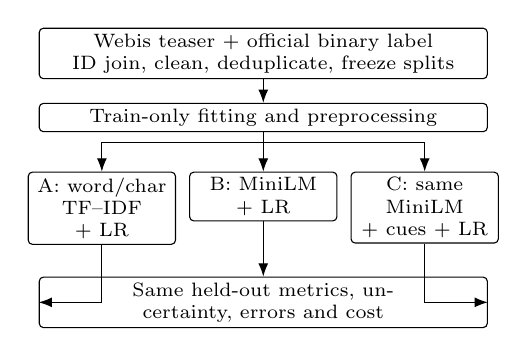
\begin{tikzpicture}[>=Latex, node distance=3mm,
  box/.style={draw,rounded corners=1.5pt,align=center,inner sep=2pt,font=\scriptsize,text width=5.55cm},
  branch/.style={draw,rounded corners=1.5pt,align=center,inner sep=2pt,font=\scriptsize,text width=1.73cm}]
\node[box] (d) {Webis teaser + official binary label\\ID join, clean, deduplicate, freeze splits};
\node[box,below=of d] (p) {Train-only fitting and preprocessing};
\node[branch,below=5mm of p,xshift=-2.05cm] (a) {A: word/char\\TF--IDF + LR};
\node[branch,below=5mm of p] (b) {B: MiniLM\\+ LR};
\node[branch,below=5mm of p,xshift=2.05cm] (c) {C: same MiniLM\\+ cues + LR};
\node[box,below=7mm of b] (e) {Same held-out metrics, uncertainty, errors and cost};
\draw[->] (d) -- (p);
\draw[->] (p.south) -- ++(0,-1.3mm) -| (a.north);
\draw[->] (p.south) -- (b.north);
\draw[->] (p.south) -- ++(0,-1.3mm) -| (c.north);
\draw[->] (a.south) |- (e.west);
\draw[->] (b.south) -- (e.north);
\draw[->] (c.south) |- (e.east);
\end{tikzpicture}
\caption{One shared evaluation pipeline. LR = logistic regression; all three branches use the same split IDs and held-out labels.}
\label{fig:pipeline}
\end{figure}

\section{Evaluation plan}
The primary outcome is \mF{}, with the \emph{paired C minus B} difference as the test of the hypothesis. We additionally report positive-class precision/recall/\(F_1\), average precision (PR ranking), Brier score and reliability diagrams, confusion matrices, computation time and peak memory. Label imbalance makes accuracy insufficient. Calibration and classification must be interpreted separately \cite{guo2017calibration}.

Three expanding-origin runs train on December, December--January, and December--February, respectively; the following month is used for validation and the next for testing. The main final comparison uses December--February for training, March for validation and untouched April for testing. We also run three fixed random grouped splits for a protocol diagnostic, and an untuned Webis-16 check if accessible. All preprocessing statistics are fitted on training data. Rather than using a fixed grid, the regularization hyperparameter \(C\) will be tuned dynamically on the validation \mF{} using randomized search to ensure fair regularization for both sparse (TF-IDF) and dense (MiniLM) representations. We will report individual temporal runs and their spread, a paired bootstrap interval for C--B on April, simple feature-group ablations, and at least 20 categorized misclassifications, including model disagreements and annotator-agreement strata. Hardware, seeds, package versions and commands will be recorded.

\section{Work plan and deliverables}
Each workstream has one \emph{accountable owner} and one \emph{supporting implementer/reviewer}; the supporting member contributes code, testing or interpretation. All four review approximately four papers each and jointly prepare the report, video, responses to feedback and Q\&A. Work division is presented in table \ref{tab:roles}

\begin{table}[]
\caption{Balanced semester workstreams. First names refer to the four named authors.}
\label{tab:roles}
\centering\scriptsize
\setlength{\tabcolsep}{3pt}
\begin{tabularx}{\columnwidth}{@{}p{1.85cm}p{1.18cm}p{1.14cm}X@{}}
\toprule
Workstream & Owner & Support & Main output\\
\midrule
Data and protocol & Adam & Igor & Clean joins, leakage-safe time splits, external data\\
Classical NLP and cues & Hubert & Adam & TF--IDF baseline, cue definitions/ablations\\
Neural NLP and hybrid & Igor & Mateusz & Frozen MiniLM, embedding and hybrid models\\
Evaluation and analysis & Mateusz & Hubert & Metrics, uncertainty, error/cost analysis, reproduction\\
\bottomrule
\end{tabularx}
\end{table}

\begin{table}[]
\caption{Weekly plan: owner(s) are accountable for the concrete completion target. Milestone dates follow the course schedule.}
\label{tab:weekly}
\centering\scriptsize
\setlength{\tabcolsep}{3pt}
\begin{tabularx}{\columnwidth}{@{}p{1.55cm}X p{1.5cm}@{}}
\toprule
Period & Completion target & Owner(s)\\
\midrule
30 Oct--4 Nov & Verify sources and data; Phase-1 proposal (4 Nov) & All; Igor edits\\
5--11 Nov & Loader, splits, TF--IDF; MiniLM cache & Adam, Hubert, Igor\\
12--18 Nov & Hybrid PoC; feedback (13 Nov); 10-min video (18 Nov) & Igor, Mateusz\\
19--25 Nov & EDA, evaluation, external-data check, Q\&A (25 Nov) & Mateusz, Adam\\
26 Nov--2 Dec & PoC merge request, revised report, rebuttal (2 Dec) & All; Igor edits\\
3--9 Dec & Apply feedback; freeze remaining tests & Hubert, Mateusz\\
10--16 Dec & Main repeated evaluation, CI, 20 errors & Igor, Mateusz\\
17--23 Dec & External check, figures and draft discussion & Adam, Hubert\\
24--30 Dec & Break / contingency; no dependency on new work & All if needed\\
31 Dec--6 Jan & Cross-reproduce best experiment; review final report & All; Adam verifies\\
7--13 Jan & Final PDF, source/MR, video and Q\&A (13 Jan) & All\\
\bottomrule
\end{tabularx}
\end{table}

\textbf{Deliverables:} (1) documented data loader and immutable split manifests with provenance; (2) reproducible three-system comparison and feature ablation with fixed metrics, uncertainty and compute costs; (3) calibration plots, at least 20 categorized errors, final report and presentation. The minimum viable outcome is a valid A--B comparison even if cues provide no measurable gain. We explicitly exclude spoiler generation, article-body verification, multilingual modelling, browser extensions and live scraping.

\section{Data statement, limitations, declarations}
\textbf{Data statement.} Webis-17 is a public, crowdsourced English social-post corpus distributed under CC BY 4.0; Webis-16 is only a proposed supplementary check pending access/reuse verification. We process teaser text and required ID/time/label fields locally, retain corpus attribution and avoid personal profiles or new scraping. Posts may contain names, handles or links; we do not enrich, rank or publish author-level identities. Released examples follow their respective dataset terms.

\textbf{Limits and risks.} The absent source IDs prevent unseen-publisher claims; temporal tests measure later periods in a historical collection, not deployment in 2026. Subjective labels, remaining topic shifts and possible pretrained-text overlap limit interpretation. The main contingency is to preserve a reproducible temporal rather than invent source groups; unavailable Webis-16 is reported rather than silently replaced.

\textbf{LLM-use declaration.} AI assistants (ChatGPT by OpenAI and Perplexity) were used for literature discovery, initial synthesis of prior work, and language verification/copyediting of the final document draft.

\begin{table}[H]
\caption{Phase-1 contribution record (completed work and actual hours); distinct from the planned semester roles.}
\label{tab:contrib}
\centering\scriptsize
\setlength{\tabcolsep}{3pt}
\begin{tabularx}{\columnwidth}{@{}p{2cm}X@{}}
\toprule
Student & Completed Phase-1 work and hours\\
\midrule
Igor Ko{\l}odziej & \IgorPhaseOne\\
Hubert Kowalski & \HubertPhaseOne\\
Adam Kaniasty & \AdamPhaseOne\\
Mateusz Iwaniuk & \MateuszPhaseOne\\
\bottomrule
\end{tabularx}
\end{table}

\begin{thebibliography}{15}
\bibitem[Potthast et al., 2016]{potthast2016}
Martin Potthast, Sebastian K\"opsel, Benno Stein, and Matthias Hagen. 2016.
Clickbait detection. In \emph{Advances in Information Retrieval (ECIR)}, pages 810--817.

\bibitem[Biyani et al., 2016]{biyani2016}
Prakhar Biyani, Kostas Tsioutsiouliklis, and John Blackmer. 2016.
``8 Amazing Secrets for Getting More Clicks'': Detecting clickbaits in news streams using article informality. In \emph{AAAI}, pages 94--100.

\bibitem[Anand et al., 2017]{anand2017}
Ankesh Anand, Tanmoy Chakraborty, and Noseong Park. 2017.
We used neural networks to detect clickbaits: You won't believe what happened next! In \emph{ECIR}, pages 541--547.

\bibitem[Wei and Wan, 2017]{wei2017}
Wei Wei and Xiaojun Wan. 2017.
Learning to identify ambiguous and misleading news headlines. In \emph{IJCAI}, pages 4172--4178.

\bibitem[Potthast et al., 2018]{potthast2018}
Martin Potthast, Tim Gollub, Kristof Komlossy, Sebastian Schuster, Matti Wiegmann, Erika Patricia Garces Fernandez, Matthias Hagen, and Benno Stein. 2018.
Crowdsourcing a large corpus of clickbait on Twitter. In \emph{COLING}, pages 1498--1507.

\bibitem[Potthast et al., 2018b]{potthast2018challenge}
Martin Potthast, Tim Gollub, Matthias Hagen, and Benno Stein. 2018.
The Clickbait Challenge 2017: Towards a regression model for clickbait strength. \emph{arXiv:1812.10847}.

\bibitem[Indurthi et al., 2020]{indurthi2020}
Vijayasaradhi Indurthi, Bakhtiyar Syed, Manish Gupta, and Vasudeva Varma. 2020.
Predicting clickbait strength in online social media. In \emph{COLING}, pages 4835--4846.

\bibitem[Yi et al., 2022]{yi2022}
Xiaoyuan Yi, Jiarui Zhang, Wenhao Li, Xiting Wang, and Xing Xie. 2022.
Clickbait detection via contrastive variational modelling of text and label. In \emph{IJCAI}, pages 4475--4481.

\bibitem[Brosco\c{t}eanu and Ionescu, 2023]{roclico2023}
Daria-Mihaela Brosco\c{t}eanu and Radu Tudor Ionescu. 2023.
A novel contrastive learning method for clickbait detection on RoCliCo: A Romanian clickbait corpus of news articles. In \emph{Findings of EMNLP}, pages 9547--9555.

\bibitem[Yu et al., 2024]{yu2024}
Jianxing Yu, Shiqi Wang, Han Yin, Zhenlong Sun, Ruobing Xie, Bo Zhang, and Yanghui Rao. 2024.
Multimodal clickbait detection by de-confounding biases using causal representation inference. In \emph{EMNLP}, pages 10300--10317.

\bibitem[An\dj eli\'c et al., 2025]{andelic2025}
Marija An\dj eli\'c, Dominik \v{S}ipek, Laura Majer, and Jan \v{S}najder. 2025.
What makes you CLIC: Detection of Croatian clickbait headlines. In \emph{Slavic NLP}, pages 116--123.

\bibitem[Michaluk et al., 2026]{michaluk2026}
Wojciech Michaluk, Tymoteusz Urban, Mateusz Kubita, Soveatin Kuntur, and Anna Wr\'oblewska. 2026.
Click it or leave it: Detecting and spoiling clickbait with informativeness measures and large language models. \emph{arXiv:2602.18171}.

\bibitem[Reimers and Gurevych, 2019]{reimers2019sbert}
Nils Reimers and Iryna Gurevych. 2019.
Sentence-BERT: Sentence embeddings using Siamese BERT-networks. In \emph{EMNLP-IJCNLP}, pages 3982--3992.

\bibitem[Wang et al., 2020]{wang2020minilm}
Wenhui Wang, Furu Wei, Li Dong, Hangbo Bao, Nan Yang, and Ming Zhou. 2020.
MiniLM: Deep self-attention distillation for task-agnostic compression of pre-trained Transformers. In \emph{NeurIPS} 33.

\bibitem[Guo et al., 2017]{guo2017calibration}
Chuan Guo, Geoff Pleiss, Yu Sun, and Kilian Q. Weinberger. 2017.
On calibration of modern neural networks. In \emph{ICML}, PMLR 70, pages 1321--1330.
\end{thebibliography}
\end{document}
